% Gated cross-attention fusion — signal-processing paper style (monochrome, tensor stacks + zero-init gate).
% Compile:  pdflatex fig_arch_gatefusion_sigproc.tex
\documentclass[border=12pt]{standalone}
\usepackage{amsmath,amssymb}
\usepackage{tikz}
\usetikzlibrary{arrows.meta,calc,positioning}
\begin{document}
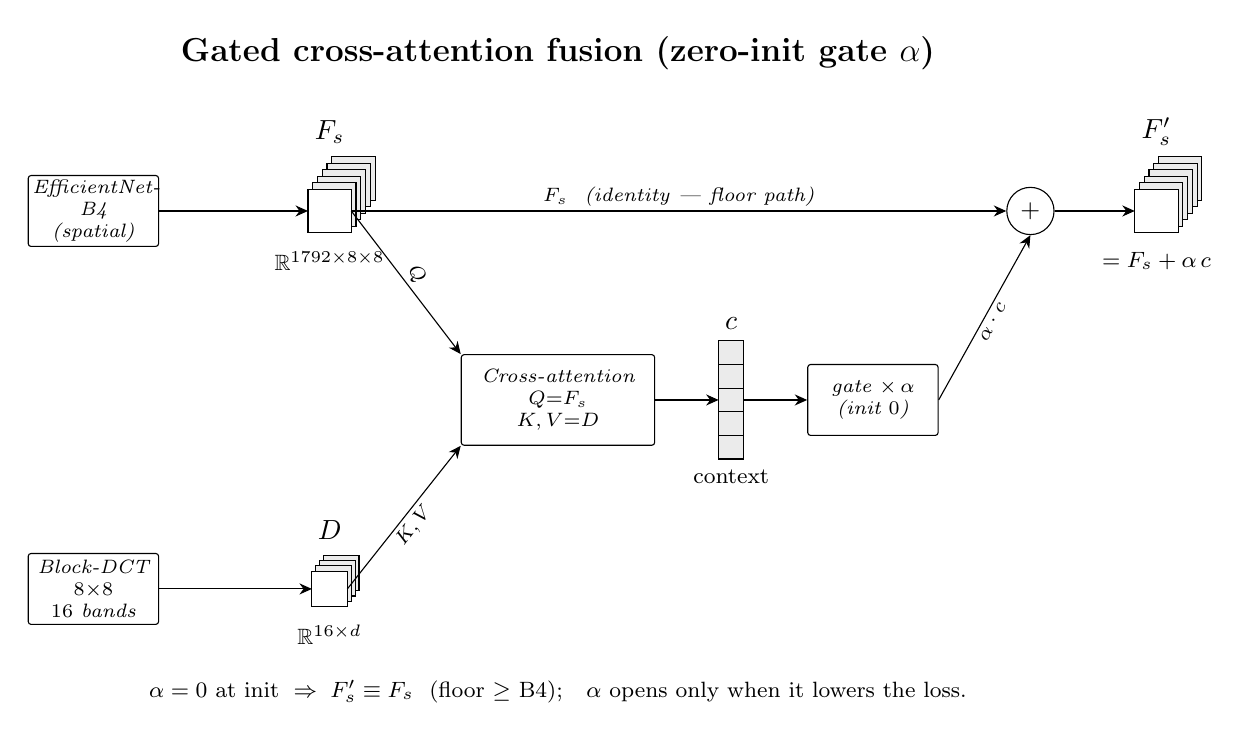
\begin{tikzpicture}[
  font=\small,
  op/.style={draw=black, thin, fill=white, rounded corners=1pt,
             text width=1.55cm, align=center, minimum height=0.9cm,
             inner sep=1.5pt, font=\scriptsize\itshape},
  bigop/.style={op, text width=2.35cm, minimum height=1.15cm},
  sumn/.style={draw=black, thin, circle, inner sep=0pt, minimum size=0.6cm, font=\small},
  arr/.style={-{Stealth[length=4.5pt,width=4pt]}, thin},
  lbl/.style={font=\scriptsize\itshape, inner sep=1.5pt},
]
% ---- tensor-stack macro: #1 id #2 x #3 y #4 n #5 side #6 above #7 below ----
\newcommand{\stk}[7]{%
  \pgfmathsetmacro{\ss}{#5}\pgfmathsetmacro{\ox}{0.11*#5}\pgfmathsetmacro{\oy}{0.15*#5}%
  \foreach \i in {#4,...,1}{%
    \pgfmathtruncatemacro{\k}{\i-1}%
    \ifnum\i=1 \def\fc{white}\else \def\fc{black!8}\fi
    \pgfmathsetmacro{\xll}{#2 - \ss/2 + \k*\ox}\pgfmathsetmacro{\yll}{#3 - \ss/2 + \k*\oy}%
    \pgfmathsetmacro{\xur}{\xll + \ss}\pgfmathsetmacro{\yur}{\yll + \ss}%
    \draw[thin,fill=\fc] (\xll,\yll) rectangle (\xur,\yur);%
  }%
  \pgfmathtruncatemacro{\kn}{#4-1}%
  \pgfmathsetmacro{\ytop}{#3 + \ss/2 + \kn*\oy + 0.32}\pgfmathsetmacro{\ybot}{#3 - \ss/2 - 0.36}%
  \pgfmathsetmacro{\xw}{#2 - \ss/2}\pgfmathsetmacro{\xe}{#2 + \ss/2}\pgfmathsetmacro{\yn}{#3 + \ss/2 + \kn*\oy}%
  \node[font=\itshape] at (#2,\ytop) {#6};\node[font=\footnotesize] at (#2,\ybot) {#7};%
  \coordinate (#1-w) at (\xw,#3);\coordinate (#1-e) at (\xe,#3);\coordinate (#1-n) at (#2,\yn);%
  \coordinate (#1-s) at (#2,#3 - \ss/2);%
}
\newcommand{\vbar}[5]{%
  \draw[thin,fill=black!8] (#2-0.16,#3-0.75) rectangle (#2+0.16,#3+0.75);%
  \foreach \t in {1,...,4}{\pgfmathsetmacro{\yt}{#3-0.75+\t*0.3}\draw[thin] (#2-0.16,\yt)--(#2+0.16,\yt);}%
  \node[font=\itshape] at (#2,#3+0.97) {#4};\node[font=\footnotesize] at (#2,#3-0.97) {#5};%
  \coordinate (#1-w) at (#2-0.16,#3);\coordinate (#1-e) at (#2+0.16,#3);%
}

% ======================= branches =======================
% spatial branch (top)
\node[op] (B4) at (1.5,2.4) {EfficientNet-B4\\(spatial)};
\stk{Fs}{4.5}{2.4}{6}{0.55}{$F_s$}{$\mathbb{R}^{1792\times8\times8}$}

% frequency branch (bottom)
\node[op] (DCT) at (1.5,-2.4) {Block-DCT $8{\times}8$\\$16$ bands};
\stk{D}{4.5}{-2.4}{4}{0.45}{$D$}{$\mathbb{R}^{16\times d}$}

% ======================= fusion core =======================
\node[bigop] (CA) at (7.4,0) {Cross-attention\\$Q{=}F_s$\\$K,V{=}D$};
\vbar{ctx}{9.6}{0}{$c$}{context}
\node[op] (G) at (11.4,0) {gate $\times\,\alpha$\\(init $0$)};

\node[sumn] (S) at (13.4,2.4) {$+$};
\stk{Ff}{15.0}{2.4}{6}{0.55}{$F_s'$}{$=F_s+\alpha\,c$}

% ======================= edges =======================
\draw[arr] (B4.east)  -- (Fs-w);
\draw[arr] (DCT.east) -- (D-w);

% Q (spatial query) into cross-attention
\draw[arr] (Fs-e) -- node[lbl,above,sloped]{$Q$} (CA.north west);
% K,V (frequency) into cross-attention
\draw[arr] (D-e)  -- node[lbl,below,sloped]{$K,V$} (CA.south west);

% floor / identity path: F_s straight to the sum (skip connection)
\draw[arr] (Fs-e) -- node[lbl,above]{$F_s$ \ (identity --- floor path)} (S.west);

% context -> gate -> sum
\draw[arr] (CA.east) -- (ctx-w);
\draw[arr] (ctx-e)   -- (G.west);
\draw[arr] (G.east)  -- node[lbl,below,sloped]{$\alpha\cdot c$} (S.south);

% sum -> fused feature
\draw[arr] (S.east) -- (Ff-w);

% ======================= title + note =======================
\node[font=\bfseries\large] at (7.4,4.4) {Gated cross-attention fusion (zero-init gate $\alpha$)};
\node[font=\footnotesize, align=center] at (7.4,-3.7)
  {$\alpha=0$ at init $\;\Rightarrow\; F_s' \equiv F_s$ \ (floor $\geq$ B4);\quad
   $\alpha$ opens only when it lowers the loss.};
\end{tikzpicture}
\end{document}
